% mainfile: ../../../../master.tex
\subsection{Quantification with Qubit\texttrademark~ dsDNA BR Assay}
% The part of the label after the colon must match the file name. Otherwise,
% conditional compilation based on task labels does NOT work.
\label{lab,qnt}
\tags{lab,qnt,cdna,dna}
\authors{cj}
%\files{}
%\persons{}

I measure the concentrations of DNA obtained by reverse transcription from RNA samples obtained with MasterPure\texttrademark~ or AllPrep kits from micro-algae cultured cells.

Also I use the Qubit\texttrademark~ dsDNA BR assay and not the ssDNA assay because last time I tried to quantify some cDNA, it failed, and I remember discussing this with Stephen and he told me it is likely that the cDNA becomes double stranded.

\begin{figure}[H] % position of the figure 
    \centering
    \caption{Illustration for the Qubit\texttrademark~ dsDNA BR assay}
    \label{fig:label}
    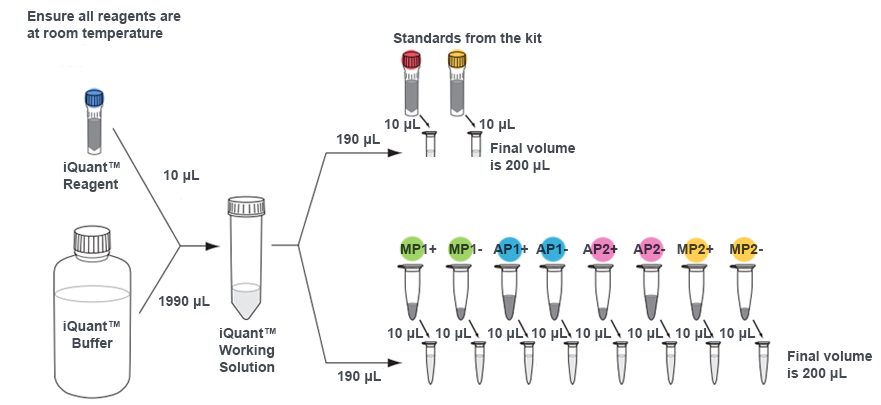
\includegraphics[width=\textwidth]{graphics/schemas/20180218_Qubit_dsDNA_assay.png}
\end{figure}

\begin{table}[H]
\caption{Total nucleic acid quantities in cDNA samples measured with Qubit\texttrademark~ Assay Kit after reverse transcription}
\label{tab:20180215_nuc_acid_qnt}
\centering
\begin{tabular}{l r r r r}
\toprule
Sample ID & \textmu g/mL & $V_f$ (mL) & m (\textmu g) & m (ng) \\ \midrule
\texttt{MP1+} & 0.335 & 0.045 & 0.015 & ~15.07 \\
\texttt{MP1-} & TOO LOW & 0.045 & - & - \\
\texttt{AP1+} & 0.331 & 0.045 & 0.014 & ~14.89 \\
\texttt{AP1-} & TOO LOW & 0.045 & - & - \\
\texttt{AP2+} & 0.501 & 0.045 & 0.022 & ~22.54 \\
\texttt{AP2-} & TOO LOW & 0.045 & - & - \\
\texttt{MP2+} & 0.663 & 0.045 & 0.029 & ~29.83 \\
\texttt{MP2-} & TOO LOW & 0.045 & - & - \\
\bottomrule
\end{tabular}
\end{table}

\comment{The cDNA concentrations are lower than what I expected so maybe it was not a smart idea to add the 30~\uL of water like it is suggested in the Protoscript First Strand Synthesis protocol. The previous time I used this protocol, I remember that I skiped this last dilution step, I should have done the same.}



